% !TeX root = ../paper.tex
\section{Introduction}\label{introduction}

Vision-language-action (VLA)
models~\citep{yu2026dm0,liu2026g05,xiaomi2026robotics1,zhang2026hyvla05,ma2026internvla15,wu2026lingbotvla2,jiang2026robottt,generalist2026gen1,generalist2026gen15,genesis2026gene265}
combine pretrained vision-language representations with action generation and have achieved strong
results in simulated and real-world manipulation. On many benchmarks, VLA success rates have
approached 98\%, seemingly suggesting that these models can act on human instructions flawlessly.


However, when evaluation moves beyond standard benchmarks toward more \textbf{open-ended
environments}, VLA policies often prove \textbf{insufficiently SMART} in following real-world
instructions. A counterintuitive example illustrates this limitation. A policy may
\textcolor{blue}{successfully} execute ``pick up the cup and place it on the plate,'' an instruction
closely resembling those in its training data, yet \textcolor{red}{fail to} follow the simpler
\textbf{fine-grained command} ``approach the cup'' or even ``move forward,'' instead producing
unrelated movements or falling back on the familiar pick-and-place routine. Similar failures arise
when users convey intent through \textbf{multimodal instructions}: given a trajectory drawn on the
image or a red circle marking the object to grasp, the policy often disregards the cue and moves
toward a familiar target. Likewise, when a robot makes an error or is about to perform an unsafe
action, a human operator may issue \textbf{corrective commands} such as ``stop'' or ``go around to
the right, not the left,'' yet the policy frequently continues along its original course. These
cases reveal a substantial gap between current VLA capabilities and genuine instruction-following
ability.



To quantify this gap, we conduct controlled behavioral interventions on three representative VLAs,
$\pi_{0.5}$~\citep{intelligence2025pi}, GR00T N1.6~\citep{gear2025gr00tn16}, and
StarVLA~\citep{community2026starvla}, using LIBERO-based manipulation tasks. As shown in
Figure~\ref{fig:overview}, all three models achieve 96--99\% complete-task success with the
original task instructions and scenes. When instructions instead specify fine-grained actions,
success drops sharply to 1--6\%. When explicit visual prompts specify the object or spatial target,
success is only 2--5\%. For corrective control, we initialize the robot in an intermediate state
with an object already held and update the target or subsequent execution requirement; success
averages only 14\% across the three models, ranging from 6\% to 25\%. These results show that even
models with strong manipulation benchmark performance remain far from sufficiently smart instruction
following.

We summarize these failures as three limitations in instruction following:
\textcircled{1}~\textbf{fine-grained semantic following}, where policies fail to execute the local
action, scope, or constraint specified by an instruction and instead default to familiar complete
tasks; \textcircled{2}~\textbf{multimodal instruction understanding}, where policies fail to ground
explicit visual prompts in the intended object, target, or motion; and
\textcircled{3}~\textbf{mid-execution corrective control}, where policies fail to revise subsequent
actions once the instruction is updated during execution. Without these capabilities, current VLA
policies are not smart enough to serve as reliable low-level controllers, hindering the translation
of high-level plans and human corrections into flexible, responsive behavior in the physical world.

% !TeX root = ../paper.tex
\begin{figure}[t]
  \centering
  \setlength{\parskip}{0pt}
  % One body-line gap before the caption; retain the standard float-to-text gap.
  \setlength{\abovecaptionskip}{\baselineskip}
  \setlength{\belowcaptionskip}{0pt}
  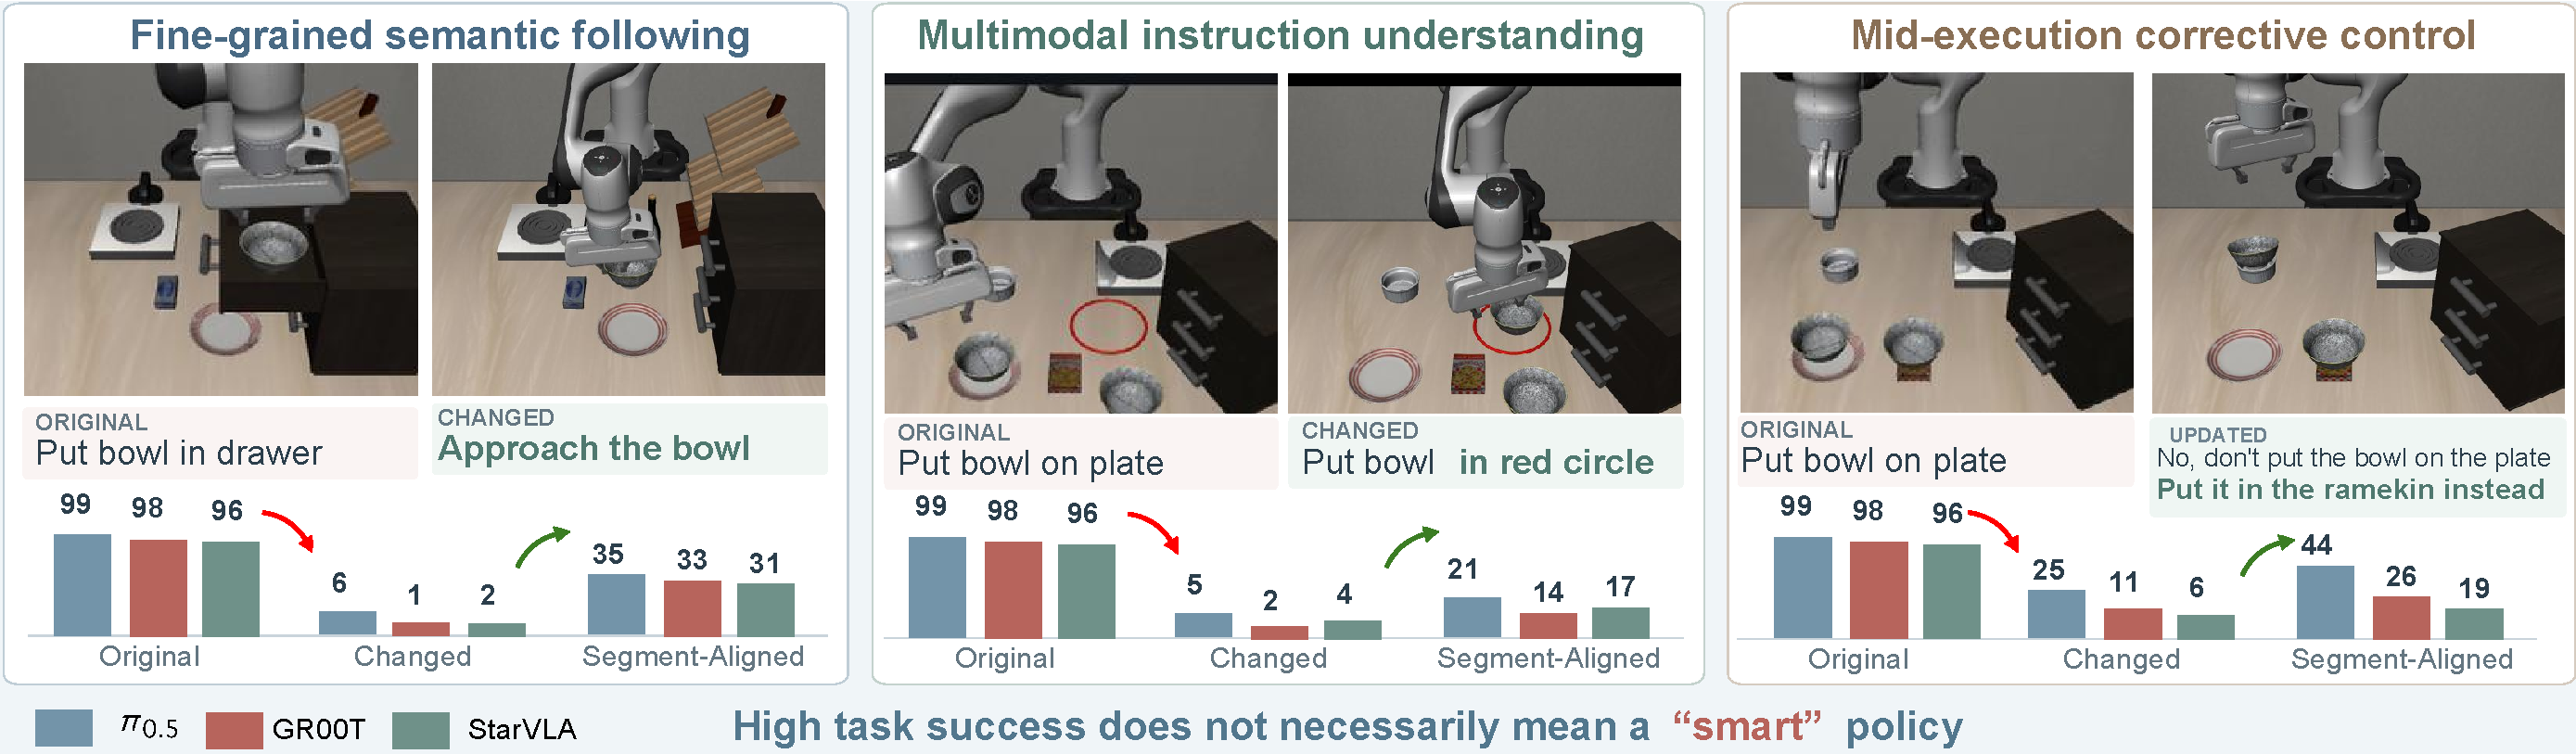
\includegraphics[width=\textwidth,pagebox=cropbox]{figures/1--figure1_editable.pdf}\par\nointerlineskip
  \caption{Instruction-following diagnosis across fine-grained semantic following, multimodal
  instruction understanding, and mid-execution corrective control. Bars compare success rates
  (\%) under original instructions, changed or updated instructions, and segment-aligned
  supervision for $\pi_{0.5}$, GR00T, and StarVLA. High original-task success can coexist with
  poor instruction following, while segment-aligned supervision improves performance under
  the changed requirements.}
  \label{fig:overview}
\end{figure}
%

%我觉得中间缺了一个东西，从现象到原因的分析，就是下面的猜想的初步验证，比如切分指令后训练确实有效果。%
% !TeX root = ../paper.tex
\begin{wrapfigure}{r}{0.48\textwidth}
  \vspace{-\intextsep}
  \centering
  \setlength{\parskip}{0pt}
  \setlength{\abovecaptionskip}{6pt}
  \setlength{\belowcaptionskip}{0pt}
  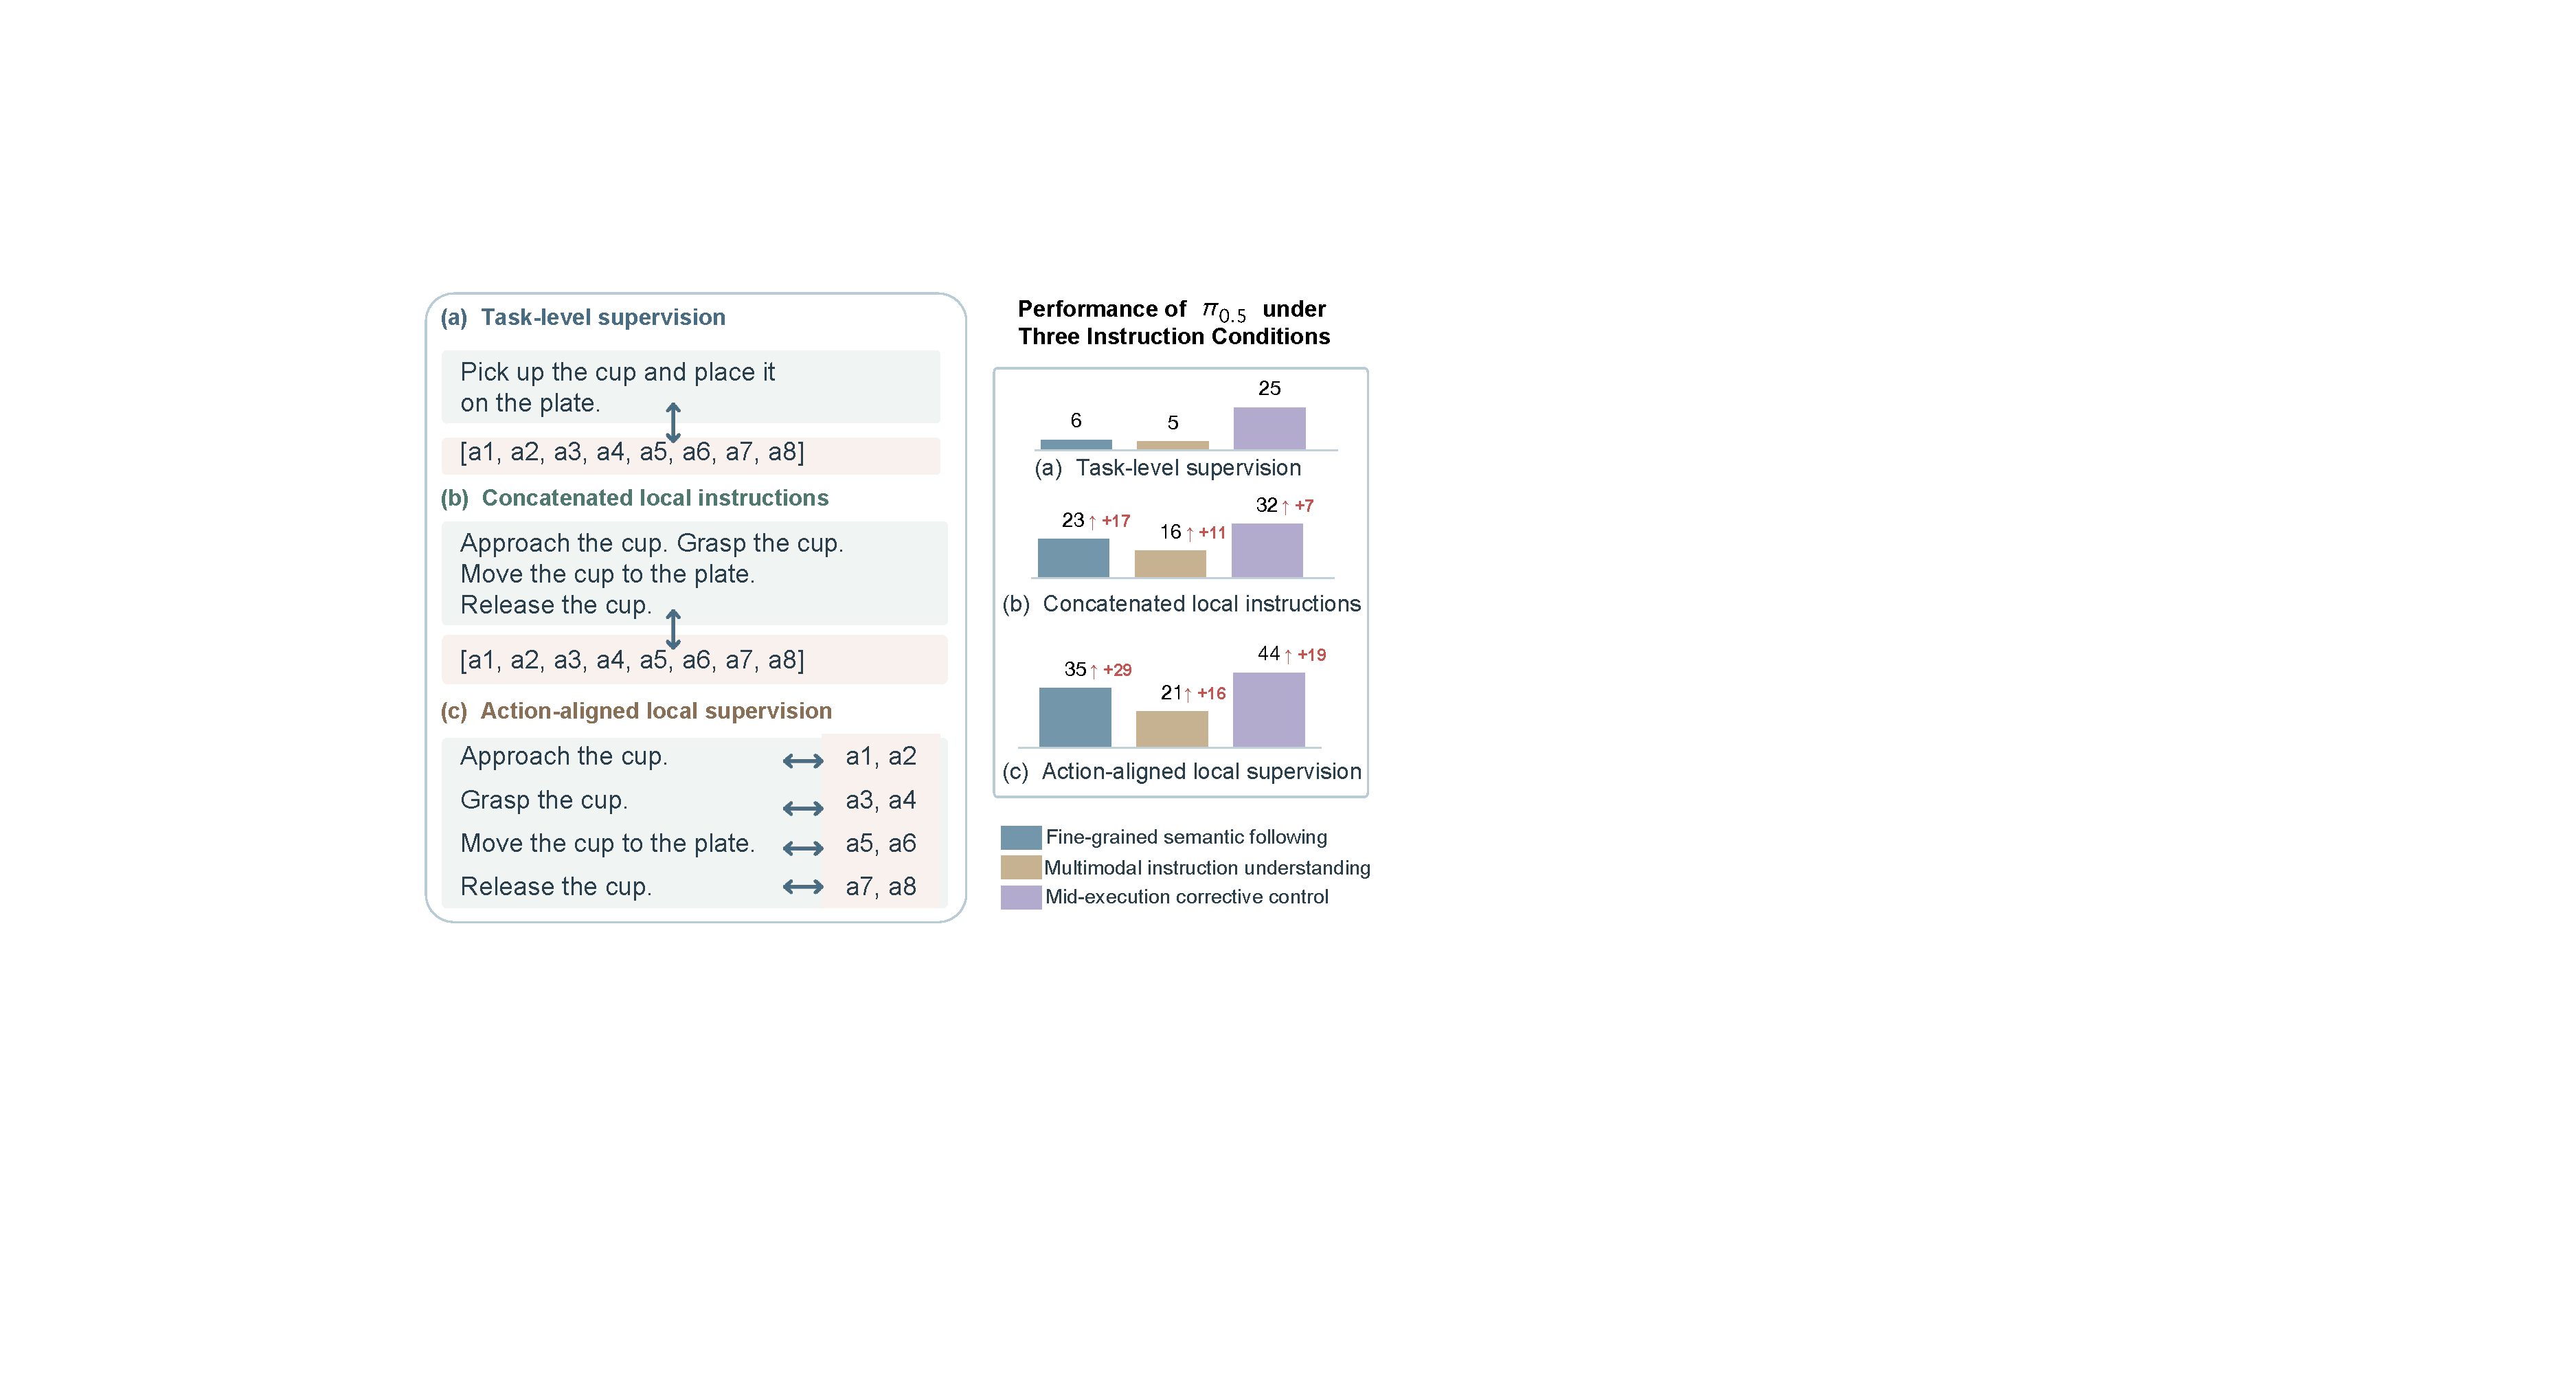
\includegraphics[width=\linewidth,pagebox=cropbox]{figures/2-fig2.pdf}\par\nointerlineskip
  \caption{Effect of supervision granularity on $\pi_{0.5}$ instruction following.}
  \label{fig:supervision-granularity}
\end{wrapfigure}
%
A plausible explanation is that task-level supervision pairs a single instruction with an entire
action sequence but provides little explicit guidance on which parts of the instruction govern
each local action. Under such supervision, a policy may rely on visual cues in familiar scenes to
reproduce action sequences without adequately using the current instruction to determine the
required local actions, thereby taking visual shortcuts that bypass instruction requirements. To
examine whether explicitly aligning local instructions with action segments improves instruction
following, we divide demonstration trajectories into $K$ consecutive local action segments based on
action phases and annotate each segment with its corresponding local instruction. As shown in
Figure~\ref{fig:supervision-granularity}, in a small-scale training comparison, we evaluate two
supervision strategies: concatenating all local instructions to supervise the entire action sequence
yields success rates of \textbf{23\%, 16\%, and 32\%} in the
fine-grained instruction, visual-prompt, and corrective-control settings, respectively; pairing each
local instruction with its corresponding action segment during training further improves these rates
to \textbf{35\%, 21\%, and 44\%}. These results indicate that richer instruction annotations improve
instruction following, while explicitly aligning local instructions with their corresponding action
segments provides additional gains beyond language enrichment alone.

% After training on such data, the model's success rates on the same interventions rise from 6\%, 5\%, and 25\% for $\pi_{0.5}$ to 54\%, 47\%, and 55\% in the fine-grained, visual-prompt, and corrective-control settings, respectively (Figure~\ref{fig:smartvla-behavior}). This suggests that supervision granularity, rather than basic manipulation ability, is a key bottleneck. 

%补充实验


% Therefore, we propose \textbf{SmartVLA} to strengthen instruction-conditioned control through coordinated data construction and training看不懂后半句. Paraphrasing an entire task can increase linguistic diversity without clarifying which actions a local command should govern 没头没尾一句话，这么做结果如何. We therefore construct supervision that binds each command and visual prompt to the corresponding control phase. 

We therefore propose SmartVLA, a framework centered on supervision that aligns local instructions
with action segments to improve fine-grained semantic following, multimodal instruction
understanding, and mid-execution corrective control in VLA policies. Motivated by the preceding
experiment on supervision granularity, we explicitly pair local instructions with action segments to
provide fine-grained supervision, rather than relying solely on a single task-level instruction for
an entire demonstration. To construct this segment-level supervision, we develop an automated
action-aligned data construction pipeline that first determines the scope of local behavior from
action and interaction evidence in demonstrations, then generates and reviews the corresponding
local instructions. By grounding instruction generation in demonstrated behavior, the pipeline
reduces reliance on costly end-to-end video annotation and per-segment manual rewriting. To further
improve multimodal instruction understanding, the pipeline also adds visual prompts to the image
observations of applicable segments to specify objects, spatial targets, or motion paths. These
prompts are paired with the corresponding local instructions and action segments to form multimodal
training examples.

However, even when local instructions are aligned with action segments, a policy may still rely
excessively on visual cues from familiar scenes without sufficiently using the current instruction
to generate actions. We therefore adopt \textbf{three training stages: warmup, pretraining, and
adaptation}. Warmup learns the correspondence between instructions and motion without image inputs;
pretraining restores visual inputs to learn how to execute instructions in the current scene; and
adaptation supports both complete-task execution and local instruction following in the target
domain. The policy can accept updated instructions in subsequent calls, allowing human operators or
upper-level models to steer ongoing execution.


To evaluate whether these capabilities are realized in existing policies, we introduce LIBERO-SMART,
which separately assesses three forms of instruction following: fine-grained semantic following,
where the policy must execute the specified local action, relation, or constraint; multimodal
instruction understanding, where visual prompts specify the current object or target location; and
mid-execution corrective control, where the policy must adapt its subsequent actions after a command
update or redirection.
Although $\pi_{0.5}$ achieves 96.85\% on the original LIBERO benchmark, its average success rate on
LIBERO-SMART is only 7.18\%. This gap is consistent with our diagnostic observations: a policy may
possess strong basic manipulation skills while failing to follow semantic requirements and visual
prompts or to redirect its behavior after an intermediate command change.

On LIBERO-SMART, SmartVLA-Pi and SmartVLA-OFT achieve average success rates of 14.67\% and 14.03\%,
respectively, compared with 7.18\% for $\pi_{0.5}$, with both variants outperforming all
direct-policy baselines across the three suites. Ablation studies support the contributions of
action-aligned segmentation, grade-conditioned rewriting, spatial supervision, and staged training
to these gains. We also evaluate standard task performance on
LIBERO, LIBERO-Plus, LIBERO-Pro, and RoboTwin, as well as real-world instruction following on the
Piper platform. SmartVLA-Pi achieves 98.30\% on LIBERO
and 84.00\% on LIBERO-Plus, outperforming $\pi_{0.5}$ by 1.45 and 3.74 percentage points,
respectively. On Piper, it raises average success from 45.00\% to 58.50\%, a gain of 13.50
percentage points. These experiments show that SmartVLA enables smarter, more flexible, and more
controllable robot behavior while maintaining strong performance on standard benchmarks.

Our contributions are:

\begin{itemize}
\item
  We develop SmartVLA to connect current instructions with local control. An action-aligned pipeline
  reconstructs existing demonstrations into phase-specific semantic and visual supervision, while
  staged training establishes a language-conditioned action prior, grounds it in observations, and
  adapts it to target domains with complete-task and local supervision.
\item
  We introduce LIBERO-SMART, comprising Semantic, Visual Prompt (Vis), and
  Control suites with 120 tasks and 6,000 evaluation instances across
  diverse initializations, to evaluate fine-grained semantic following,
  multimodal instruction understanding, and mid-execution corrective control.
\item
  We systematically evaluate standard task performance and the three
  instruction-following capabilities across two VLA architectures on
  the LIBERO benchmarks, RoboTwin Full and C2R, LIBERO-SMART, and the
  Piper real-robot platform. We further assess callability under a
  fixed upper-level protocol.
\end{itemize}

